\apendice{Documentación técnica de programación}

\section{Introducción}
Este apéndice muestra las herramientas necesarias para entender y poder reutilizar el software presentado. Sin embargo, no es necesario utilizar las mismas herramientas, pero es muy recomendable.
Para el desarrollo del trabajo se ha utilizado MCUXpresso. A continuación se muestra cómo instalar y configurar este IDE. Además, también veremos otras herramientas que nos ayudarán a comprobar el correcto funcionamiento del software.

\section{Estructura de directorios}
Antes de comenzar la instalación de MCUXpresso veamos de que ficheros disponemos en este proyecto.
La estructura de directorios es:

\begin{figure}[!h]
	\centering
	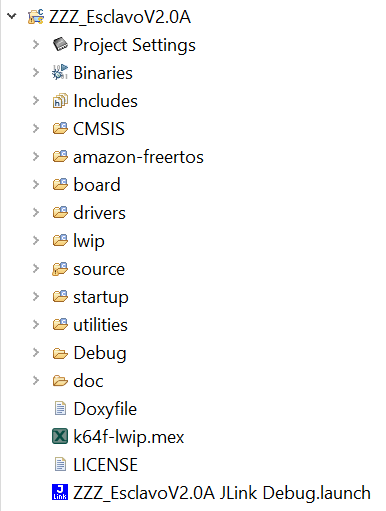
\includegraphics[width=0.5\textwidth]{directorios}
	\caption{Estructura de directorios.}
\end{figure}
\FloatBarrier

\begin{description}
  \item[/] Directorio raíz, contiene el resto de los directorios. Se incluyen ficheros como LICENSE que contiene los términos y condiciones del licenciamiento del software y el fichero .MEX que contiene los datos de las configuraciones de los pines, relojes y periféricos. Este último fichero lo genera el propio IDE. En la raíz también encontramos los archivos binarios para la ejecución del programa y el archivo para realizar el debug.
  \item[/CMSIS/] Cortex Microcontroller Software Interface Standard (CMSIS). Reúne las fuentes que proporcionan interfaces al procesador y sus periféricos.
  \item[/amazon-freertos/] Fuentes relacionadas con FreeRTOS, sistema operativo en tiempo real usado en el proyecto.
  \item[/board/] Fuentes autogenerados por el IDE que permiten habilitar y configurar el hardware de la placa de desarrollo.
  \item[/doc/] Documentación del proyecto.
  \item[/drivers/] Controladores necesarios para trabajar con el hardware.
  \item[/lwip/] Fuentes relativos a lwIP, la implementación de la pila de protocolos TCP/IP.
  \item[/source/] Código fuente del proyecto. El fichero main.c es el que contiene el código del funcionamiento de las placas. Además se encuentran los ficheros que agrupan herramientas para completar la ejecución de las funciones utilizadas en el main.c.
  \item[/startup/] Código de arranque generado por el IDE.
  \item[/utilities/] Código generado por el IDE con utilidades auxiliares usadas para depuración o registro de eventos.
\end{description}

\section{Manual del programador}
\subsection{Descarga e instalación de MCUXpresso}
En primer lugar será necesario descargar el IDE desde la página oficial de NXP. Este software estará en la pestaña de desarrolladores. Para poder descargarlo será necesario tener una cuenta de NXP, la cual es gratuita y te puedes registrar fácilmente desde el sitio web.
Dicho esto, iniciamos sesión en la página vamos a la pestaña en la que se encuentra el software y pinchamos en descargar \cite{DLMCUX}. 

\imagen{DIDLE}{Pagina de descarga del IDE.}

Una vez hecho esto, elegimos el sistema operativo donde se ejecutará nuestro IDE. El instalador sigue los pasos habituales en este tipo de instalaciones, aceptar la licencia, elegir la ubicación donde se guardarán los archivos y controladores de programa, etc. Podemos dejar todas estas opciones por defecto o variarlas a nuestro gusto. 
Al descargar el IDE viene con él la herramienta Config Tools que nos ayudará a realizar la configuración a bajo nivel de la placa. 



Una vez tenemos instalado MCUXpresso, lo abrimos. Lo primero que nos pide es elegir una ruta donde guardar nuestros proyectos. Es recomendable que sea una ruta fácilmente accesible pues nos será de gran ayuda poder llegar rápidamente y poder importar y exportar de manera más sencilla los proyectos que necesitemos.

\begin{figure}[!h]
	\centering
	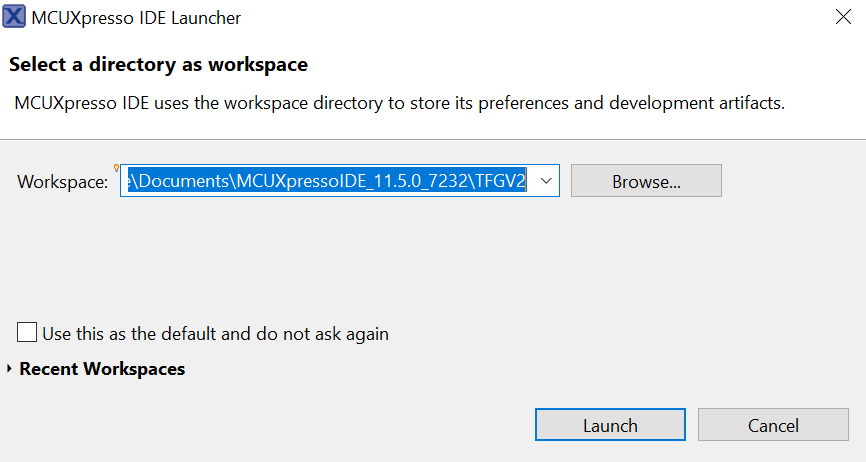
\includegraphics[width=0.6\textwidth]{rutaProyectoIde}
	\caption{Elección de la ruta para guardar los proyectos en local.}
\end{figure}
\FloatBarrier

Tras elegir la ruta y pulsar `Launch' encontraremos la siguiente interfaz:

\imagen{IntPrincMCUXpresso}{Interfaz principal MCUXpresso.}

Como se puede apreciar en la figura anterior, el IDE proporciona una interfaz semejante al IDE Eclipse.


\subsection{Descarga e instalación del SDK}
Tras esta instalación del IDE, deberemos realizar el segundo paso en el que descargaremos el SDK. Podemos descargarlo también desde la web de NXP \cite{DLSDK}, en esta pestaña deberemos elegir el SDK correspondiente a la placa y comprobar que la versión sea superior a la 2.0. \\
A la hora de descargar el SDK es recomendable seleccionar todos sus paquetes por si los necesitáramos para futuros proyecto pero en caso de que no queramos descargarlos ahora podremos elegir solo algunos y descargarlos a `posteriori' según los vayamos necesitando. Mínimo deberemos descargar FreeRTOS y CMSIS.

\imagen{sdk}{Pagina de descarga del SDK para la placa K64F.}

La descarga del SDK nos permite construir proyectos específicos para nuestra placa, permite además añadir los componentes necesarios según las funcionalidades del SE. Nos ofrece la posibilidad de descargar e instalar drivers, el tipo de sistema operativo o configurar el middleware. En nuestro caso deberemos seleccionar como mínimo el sistema operativo FreeRTOS y como drivers lwIP y ADC para la medición del sensor de temperatura y la lectura de los potenciómetros. Para poder elegir estos add-ons deberemos clicar donde se muestra en la Figura \ref{clickSDK}.

\begin{figure}[!h]
	\centering
	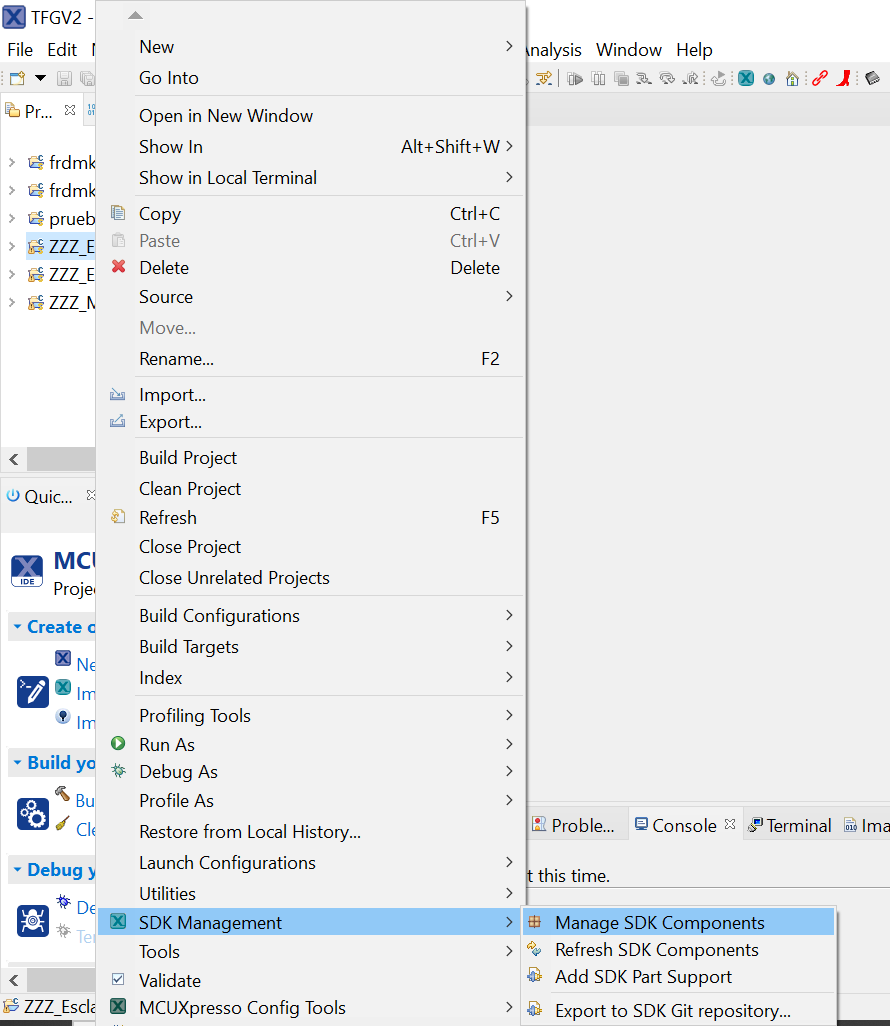
\includegraphics[width=0.6\textwidth]{GotoSDK}
	\caption{Abrir el SDK.}
	\label{clickSDK}
\end{figure}
\FloatBarrier

Posteriormente se abrirá un interfaz como la de la Figura \ref{UsingSDK}.

\imagen{UseSDK}{Elección de los Drivers necesarios.} \label{fig:UsingSDK}


Donde podremos elegir los componentes que queramos. Como se ve en la figura disponemos de un menú con distintas opciones: \extranjerismo{drivers, utilities, middleware.} Además la interfaz cuenta con una barra de buscador que nos facilita el trabajo.

\subsection{Importación del proyecto}
Importar un proyecto es bastante sencillo. Para ello iremos al repositorio de GitHub de este proyecto y descargamos los tres proyectos que componen el sistema en un `.zip'. Una vez descargados tan solo tendremos que pulsar en la opción 'import project from file system' que aparece en la Figura \ref{fig:import}:

\imagen{ImportacionProyecto}{Importación de un Proyecto.} \label{import}

Seleccionamos la ruta del proyecto o el archivo `.zip' y pulsamos en `finish'. De esta manera ya tendríamos el proyecto importado en nuestro IDE. En caso de hacerlo con el `.zip' nos saldrá otra pantalla más, en la que mi recomendación es que marquemos la opción de copiar el proyecto en la ruta de proyecto que elegimos previamente.

\subsection{ConfigTools: Configuración de pines, relojes y periféricos}
La configuración a bajo nivel de la placa es una de las partes más importantes y a la vez más complejas de entender al principio, por ello voy a explicar brevemente cómo funcionan estas interfaces del IDE.

\begin{description}
\item[Pines] Estas placas disponen de varios pines que son configurables permitiendo así la integración de varios periféricos y aumentando su funcionalidad. En la siguiente figura podemos observar la interfaz para configurarlo:

\imagen{PinesMCUX}{Interfaz de los Pines en MCUXpresso.}

En la parte izquierda de la figura vemos la lista de todos los pines que podemos configurar, que en el caso de esta placa son más de 100. Cada uno de estos pines tiene distintas configuraciones que podremos elegir según nuestras necesidades. \\ 
En la parte inferior nos muestra la lista de pines que ya hemos seleccionado y configurado. \\
Por último, en la parte de la derecha tenemos la imagen del controlador con todos sus pines. Los pines que ya se está utilizando aparecen remarcados en verde.
\item[Relojes] En el caso de este software se ha utilizado siempre el reloj configurado por defecto pero podemos configurar más relojes dependiendo del objetivo del periférico que vaya a usarlo. La Figura \ref{fig:relojes2} nos muestra una imagen de la interfaz.

\imagen{RelojesMCUX2}{Interfaz de la tabla de los Relojes en MCUXpresso.} \label{relojes2}

En la figura anterior se ven los relojes asignados a distintos elementos de la placa y en la parte izquierda los asignados a los periféricos. Estos relojes se pueden cambiar en un rango de frecuencias que se muestran en el diagrama de relojes de la Figura \ref{fig:relojes1}.
\imagen{RelojesMCUX}{Interfaz del diagrama de los relojes en MCUXpresso} \label{relojes1}

\item[Periféricos] el microcontrolador permite conectar varios periféricos a la placa al mismo tiempo. En la Figura \ref{fig:perifericos} se muestran cuales son:

\imagen{PerifericosMCUX}{Interfaz de los Periféricos en MCUXpresso.} \label{perifericos}

Como se puede apreciar, hay algunos repetidos como por ejemplo UART puesto que esta placa permite tener hasta 4 comunicaciones UART configurables al mismo tiempo. En algunas ocasiones, podría darse el caso de que no se puedan añadir más periféricos de esta lista porque los pines que son configurables para ese fin están siendo utilizados, aunque esto solo pasara en casos de sistemas SE muy concretos. \\
Cada una de las configuraciones de los periféricos tiene sus correspondientes opciones específicas. Estas configuraciones nos ayudan para que no tengamos que configurarlas programando y solo tengamos que hacer `click’ o elegir algunas de ellas. 
\end{description}

\section{Compilación, instalación y ejecución del proyecto}\label{sec:compilacion}

Una vez que hemos importado el proyecto, vamos a la carpeta sources y vemos que el fichero tiene los datos fuente del proyecto. Para poder compilar clicaremos en la opción \extranjerismo{build} para ver si el proyecto compila adecuadamente o tiene errores.

\begin{figure}[!h]
	\centering
	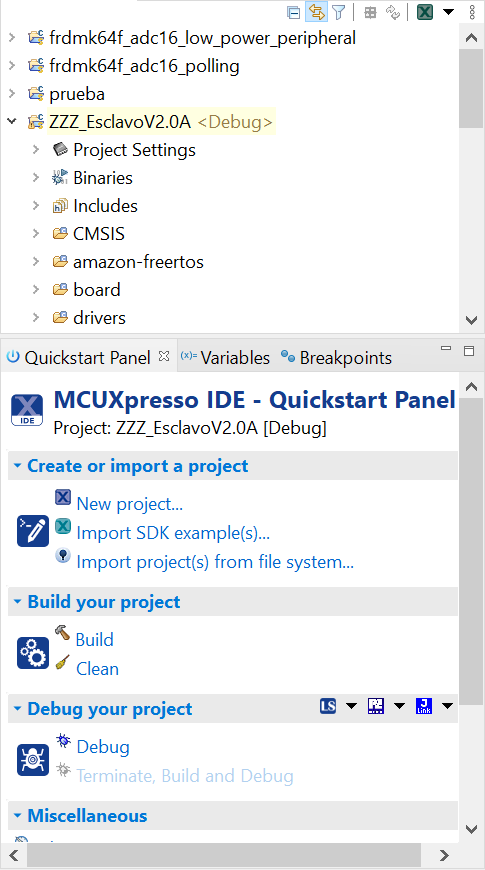
\includegraphics[width=0.5\textwidth]{compilacion}
	\caption{Compilación del Proyecto.}
\end{figure}
\FloatBarrier

Posteriormente deberemos conectar por USB la placa FRDM K64F al ordenador. Antes de seguir con el \extranjerismo{debugueo}, es importante que la placa esté en modo OpenSDA, para ello, si es la primera vez que la usamos, deberemos pulsar el botón reset mientras conectamos la placa al ordenador. Tras esto se debería de abrir una carpeta llamada `bootloader' donde deberemos copiar el fichero openSDA. Desconectamos y conectamos la placa de nuevo y la placa quedaría lista para realizar la escritura, o flash, de los archivos binarios del proyecto. 
Para este paso debemos pulsar la opción `debug' para iniciar la depuración. Una vez comience la ejecución se abrirá una consola y podremos utilizar el SE sin problemas. La primera vez que usemos una placa el IDE nos solicita la identificación de la misma. Para ello deberemos seleccionar el uso de `Segger J-Link Probes' que es compatible con OpenSDA y el adaptador serie y de depuración que viene integrado en la placa.

Dicho esto, es importante recalcar que estos métodos para compilar y depurar el programa no son los únicos, puesto que en el IDE se disponen de varios menús que en ocasiones repiten las mismas funcionalidades. Como dato a tener en cuenta, es interesante saber que la ejecución de la opción debug trae consigo la compilación del proyecto de manera automática si no se realizó manualmente antes de ejecutarse.

\section{Distribución de pines} \label{distribucionDePines}
En este apartado se muestran los pines usados para la comunicación de la pantalla LCD y de los motores. En la figura \ref{pinesUsados} se muestran los pines de la placa FRDM K64F.

\begin{figure}[!h]
	\centering
	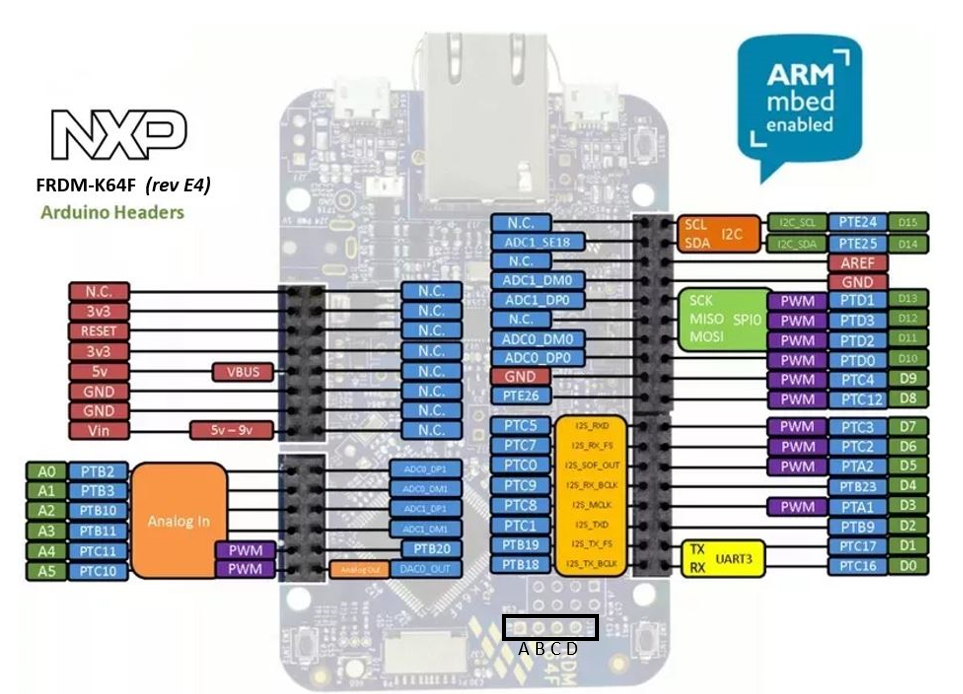
\includegraphics[width=0.9\textwidth]{pinesUsados}
	\caption{Definición de los pines de la placa FRDM K64F.}\label{pinesUsados}
\end{figure}

La figura \ref{ayudaPines} muestra las conexiones de la pantalla LCD y la placa controladora de los motores para poder entender mejor las siguientes tablas.

\begin{figure}[!h]
 \centering
  \subfloat[Módulo I2C LCD]{
    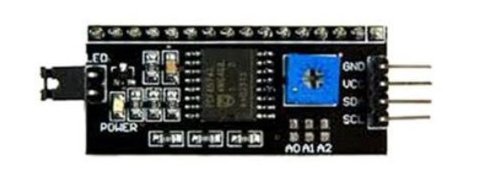
\includegraphics[width=0.5\textwidth]{moduloLCD.png}}
  \subfloat[Controladora MD25]{
    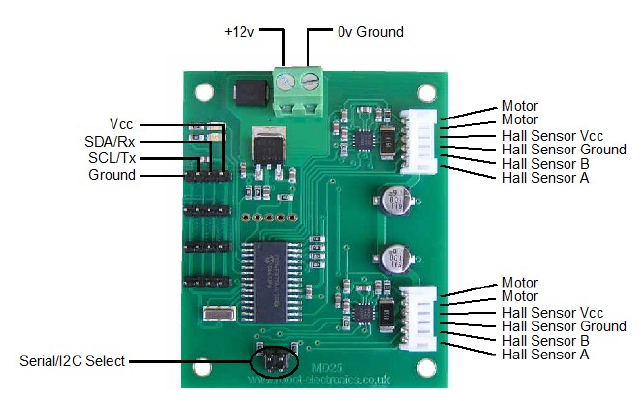
\includegraphics[width=0.5\textwidth]{placaMotor.png}}
 \caption{Conexión de Pines}\label{ayudaPines}
\end{figure}

\newpage

Los pines de la pantalla LCD se conectarán a los pines de la placa especificados en la tabla \ref{tabla:pinesLCD}\\

\tablaSmallSinColores{Pines FRDM K64F y pantalla LCD.}{c c}{pinesLCD}
{\multicolumn{1}{c}{ Pin K64F } & Pin Pantalla LCD\\}
{
PTE24 & SCL \\
PTE25 & SDA \\
5V & VCC \\
GND & TIERRA \\
}

En la parte inferior de la figura \ref{pinesUsados} hay cuatro pines marcados con las letras: A,B,C,D, a los que se conectaran a la placa controladora de los motores. En la tabla \ref{tabla:pinesMotor} se muestra su disposición.

\tablaSmallSinColores{Pines FRDM K64F y motores EMG30.}{c c}{pinesMotor}
{\multicolumn{1}{c}{ Pin K64F } & Pin Motor EMG30\\}
{
A: 3v & VCC \\
B: Tierra & GND \\
C: PTC14, UART, RX & TX \\
D: PTC15, UART, TX & RX \\
}

\section{Pruebas del sistema: Packet Sender}
Otra herramienta que puede ayudar enormemente a los desarrolladores es packet sender. Para descargarla tendremos que ir a su página web oficial \cite{DLPS} y descargar la herramienta para el sistema operativo donde vayamos a utilizarla. Packet Sender permite enviar paquetes por el protocolo tcp, a una ip y un puerto determinados. Además se pueden guardar nuestros propios comandos de envío para reutilizarlos de forma más sencilla. De esta forma, conseguimos poder comprobar si las placas reciben los comandos adecuadamente y cómo se comportan al recibirlo. Es como tener otra placa en red pero los comandos se envían de forma más sencilla desde nuestro propio ordenador.

\imagen{packetSender}{Interfaz de la herramienta Packet Sender.}


